\documentclass[
12pt,
a4paper, 
%oneside, % Uncomment this for digital
twoside,  % Use twoside for printing.
openright, % Uncomment this for printing
]{book}
% ]{scrbook}

% Ragged bottom prevents variable spacing text and floats (done usually to keep last lines in both pages same in book format.)
\raggedbottom

% Fonts
\usepackage[english]{babel}
\usepackage{fontspec}
\usepackage{parskip}

% Bibliography
\usepackage[round]{natbib}
\usepackage[sectionbib]{chapterbib} %References on each chapter
\usepackage{chapterbib}

% Graphics and other packages for text and figures
\usepackage{graphicx}
\graphicspath{ {figures/cropped/} }
\usepackage[dvipsnames]{xcolor}
\usepackage{enumitem, siunitx, mathtools, amsfonts}
\usepackage[font=small, labelfont=bf, singlelinecheck=false, width=.95\textwidth, labelsep=colon]{caption}
\usepackage[rightFloats, CaptionBefore]{styles/fltpage}
\newtagform{brackets}{[}{]}
\usetagform{brackets}
\newcommand{\figuretitle}{}
\DeclareCaptionFormat{myformat}{#1 #2 \textbf{\figuretitle} \\ #3}
\captionsetup{format=myformat}
\captionsetup[FPfigure]{format=myformat}
\newenvironment{Mfigure}[1]
	{\renewcommand{\figuretitle}{#1}
	\begin{figure}[htbp]}
	{\end{figure}}
\newenvironment{MFPfigure}[1]
	{\renewcommand{\figuretitle}{#1}
	\begin{FPfigure}}
	{\end{FPfigure}}	
\usepackage{subcaption}

% Packages to make the thesis beautiful.
\usepackage{standalone} % load only in the main file
\usepackage{fancyhdr} %For header
\usepackage{emptypage} % Removes header from empty pages
\usepackage{longtable} % Multipage Tables
\usepackage{makeidx} %To make index page
\usepackage[totoc]{idxlayout} %To get index into TOC
\usepackage[acronym,toc]{glossaries} %Acronyms, TOC option will add it to TOC
\usepackage[titletoc,title]{appendix} %For Appendix
% \raggedbottom
% \setlength{\parskip}{1em plus .1em minus 1.em}

% Short chapter and section headings
\newcommand{\markedchapter}[2]{\chapter[#2]{#2%
\chaptermark{#1}}
\chaptermark{#1}}
\newcommand{\markedsection}[2]{\section[#2]{#2%
\sectionmark{#1}}
\sectionmark{#1}}

% Need to remove section numbers of appendix from TOC
\usepackage{etoolbox}
\appto\appendix{\addtocontents{toc}{\protect\setcounter{tocdepth}{0}}}
% reinstate the correct level for list of tables and figures
\appto\listoffigures{\addtocontents{lof}{\protect\setcounter{tocdepth}{1}}}
\appto\listoftables{\addtocontents{lot}{\protect\setcounter{tocdepth}{1}}}

%Create new style to add header on each page
\pagestyle{fancy}
\fancyhf{}
\renewcommand{\chaptermark}[1]{\markboth{#1}{}}
% \newcommand{\mymark}{\chaptername\ \thechapter.\ \ \leftmark}
\makeatletter
\fancyhead[RO]{\if@mainmatter \slshape\nouppercase{\leftmark} \else \slshape\nouppercase{\leftmark} \fi}
\fancyhead[LE]{\if@mainmatter \slshape\nouppercase{\rightmark} \else \slshape\nouppercase{\leftmark} \fi}
\makeatother
\cfoot{\fancyplain{}{\thepage}}
\setlength{\headheight}{15pt}

% Footnote related command
\newcommand\pubnote[1]{%
	\begingroup
	\renewcommand\thefootnote{}\footnote{#1}%
	\addtocounter{footnote}{-1}%
	\endgroup
}

% Author, title information
\author{C.M.O.T Dibbler}
\usepackage[
pdfauthor={C.M.O.T Dibbler},
pdftitle ={The chronicles of Blind Io},
pdfsubject={Theology},
pdfkeywords={preach, time, faith, disbelief, bargain}, hidelinks]{hyperref} %References and hyperlinks

% Comment following Hypersetup during printing
\hypersetup{ 
	colorlinks   = true, %Colours links instead of ugly boxes
	urlcolor     = blue, %Colour for external hyperlinks
	linkcolor    = BurntOrange, %Colour of internal links
	citecolor   = teal %Colour of citations
}

% \makeindex %Makes index file.
% \makeglossaries %Make glossary file

\begin{document}

	\frontmatter
	\begin{titlepage}
	\centering
	\vfill
	{\huge\bfseries The chronicles of Blind Io. \par}
	\vspace{2cm}
	{\Large A Thesis\par}
	\vfill
	Submitted to the\par
	{\Large The temple of Ankh-Morpork\par
	for the degree of Doctor of Theosophology\par}
	\vspace{1cm}
	by\par
	\vspace{0.5cm}
	{\Large \bfseries C.M.O.T Dibbler\par}
	\vfill
	
	% Bottom of the page
	{\large The temple of Ankh-Morpork\par
		Ankh-Morpork, Discworld\par}
	{October, 229018}
\end{titlepage}
	\chapter[Declaration]{\centering Declaration}
This fiction is a presentation of my original research work. Wherever contributions of others are involved, every effort is made to indicate this clearly, with due reference to the literature, and acknowledgement of collaborative research and discussions. 
\\
The work was done under the guidance of Captain Carrot Ironfoundersson, at the temple of Ankh-Morpork.
\\\\\\\\
\null\hfill \textbf{ C.M.O.T Dibbler}\\
\null\hfill The temple of Ankh-Morpork, Ankh-Morpork, Discworld
\\\\\\\\
In my capacity as supervisor of the candidate’s thesis, I certify that the above statements are true to the best of my knowledge.
\\\\\\\\
\null\hfill \textbf{Captain Carrot Ironfoundersson}\\
\null\hfill  The temple of Ankh-Morpork, Ankh-Morpork, Discworld\\
\\
\null\hfill \textbf{Date} : \qquad\qquad\qquad\qquad\qquad\\
	\chapter[Certificate]{\centering Certificate}
I certify that this thesis entitled “\textbf{The chronicles of Blind Io.}” comprises fictive work carried out by \textbf{C.M.O.T Dibbler} at Diskworld under the supervision of \textbf{Captain Carrot} during the period 2012 - 2018 for the degree of Doctor of Theosophology. The results presented in this thesis have not been submitted previously to this or any other world for a PhD or any other degree.
\\\\\\\\\\\\\\\\
\null\hfill \textbf{Head of Fiction}\\
\null\hfill Ankh-Morpork\\
\null\hfill Discworld\\

	\chapter[Publication]{\centering Publication}

\textbf{Dibbler, C.M.O.T}, Ironfoundersson, Carrot. The chronicles of Blind Io.\textit{ Fiction?}. 229018 Oct.
\\\\
{\footnotesize Content from the above publication has been incorporated in the thesis with permission from the publisher.}
	\chapter[Acknowledgments]{\centering Acknowledgments}

Captain Carrot Ironfoundersson for his forthrightness and Commander Samuel Vines for persecacity. And of course, the Rohit Suratekar of sphereworld (a.k.a Earth) for bestowing me a barebone version of this manuscript in papyrus.


	% For this page we need to remove chapter title and space above the title

% Following definition will remove the chapter title
\makeatletter
\newcommand{\unchapter}[1]{%
	\begingroup
	\let\@makechapterhead\@gobble % make \@makechapterhead do nothing
	\chapter*{#1}  % Used * so that it won't appear in Table of Content
	\endgroup
}
\makeatother

%Adjust Vspace to shift chapter above so that without title it will look like middle of the space 
\unchapter{\vspace{-5cm}} 

% Make sure to use closed center enviornment instead \centering 
%else all other chapters will also become center
\begin{center}
	\topskip0pt
	\vspace*{\fill}
	{\large Dedicated to all \par}
	\vspace{0.5cm}
	{\LARGE whatever you want!}
	\vspace*{\fill}
\end{center}

% Following will remove the page number
\thispagestyle{empty}


	\printglossary[type=\acronymtype,title={Abbreviations}, style=alttree]
	\phantomsection
	\addcontentsline{toc}{chapter}{\listfigurename}
	\listoffigures
	\phantomsection
	\addcontentsline{toc}{chapter}{\listtablename}
	\listoftables
	\tableofcontents

	\chapter{Acknowledgements}
	I would like to thank my supervisors, Professor Someone. This
	research was funded by the Imaginary Research Council.

	\chapter{Abstract}
	A brief summary of the project goes here.
	% A glossary and list of acronyms may go here
	% or may go in the back matter.

	\mainmatter
\markedchapter{Lorem Ipsum}{Introduction: Lorem Ipsum}\label{chapter-1}

\hypertarget{section-1.1}{%
\section{Section}\label{section-1.1}}

\hypertarget{eaque-ipsa-quae-ab-illo-inventore-veritatis-et-quasi.}{%
\subsection{Eaque ipsa quae ab illo inventore veritatis et
quasi.}\label{eaque-ipsa-quae-ab-illo-inventore-veritatis-et-quasi.}}

Qui officia deserunt mollit anim id est laborum. Lorem ipsum dolor sit
amet, consectetur adipisicing elit. Non numquam eius modi tempora
incidunt ut labore et dolore magnam aliquam quaerat voluptatem. Ut enim
ad minim veniam, quis nostrud exercitation ullamco
\citep{Zongkerchicken2005}. \textbf{Sed ut perspiciatis unde omnis iste
natus error sit voluptatem.} \emph{Facere possimus, omnis voluptas
assumenda est, omnis dolor repellendus.} Facere possimus, omnis voluptas
assumenda est, omnis dolor repellendus \citep{upper1974unsuccessful}.

\begin{Mfigure}{Lorem Ipsum}
 \centering
 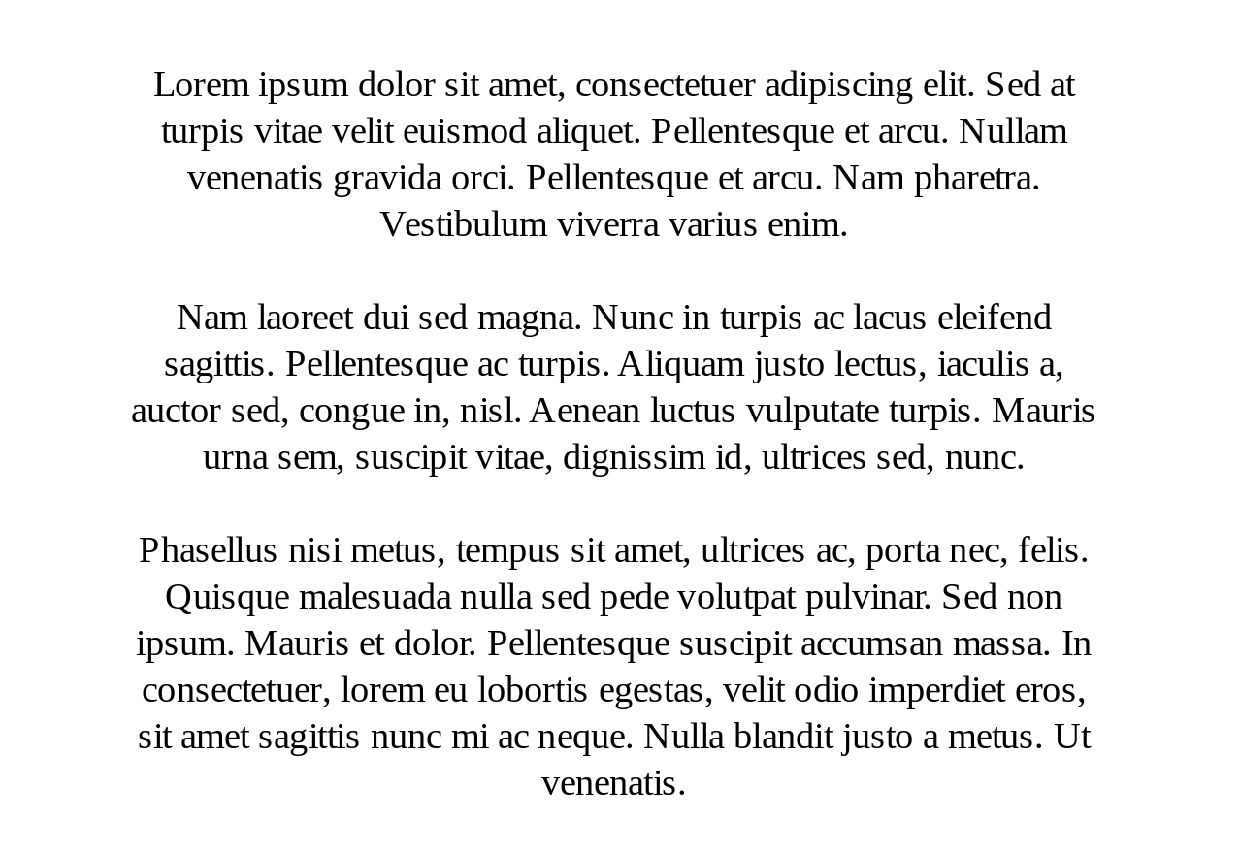
\includegraphics[width=\linewidth]{Figure-C1.pdf}
 \caption[\figuretitle]
{\textbf{(A) Lorem Ipsum.} Add as much text here as you want.}
\label{fig:c1}
\end{Mfigure}



\hypertarget{neque-porro-quisquam-est-qui-dolorem-ipsum-quia-dolor-sit-amet-consectetur-adipisci-velit.}{%
\subsubsection{Neque porro quisquam est, qui dolorem ipsum quia dolor
sit amet, consectetur, adipisci
velit.}\label{neque-porro-quisquam-est-qui-dolorem-ipsum-quia-dolor-sit-amet-consectetur-adipisci-velit.}}

Laboris nisi ut aliquip ex ea commodo consequat. Accusantium doloremque
laudantium, totam rem aperiam, eaque ipsa quae ab illo. Fugiat quo
voluptas nulla pariatur? Totam rem aperiam. At vero eos et accusamus. Et
harum quidem rerum facilis est et expedita distinctio. Et iusto odio
dignissimos ducimus qui blanditiis praesentium voluptatum deleniti
atque. Et harum quidem rerum facilis est et expedita distinctio.

\hypertarget{et-harum-quidem-rerum-facilis-est-et-expedita-distinctio.}{%
\paragraph{\texorpdfstring{Et harum quidem rerum facilis est et expedita
distinctio.\newline}{Et harum quidem rerum facilis est et expedita distinctio.}}\label{et-harum-quidem-rerum-facilis-est-et-expedita-distinctio.}}

Neque porro quisquam est, qui dolorem ipsum quia dolor sit amet,
consectetur, adipisci velit. Animi, id est laborum et dolorum fuga.
Inventore veritatis et quasi architecto beatae vitae dicta sunt
explicabo. Et harum quidem rerum facilis est et expedita distinctio.
Nihil molestiae consequatur, vel illum qui dolorem eum. Nam libero
tempore, cum soluta nobis est eligendi optio cumque nihil impedit quo
minus id quod maxime placeat. Eaque ipsa quae ab illo inventore
veritatis et quasi. Ut enim ad minim veniam, quis nostrud exercitation
ullamco. Qui officia deserunt mollit anim id est laborum. Et iusto odio
dignissimos ducimus qui blanditiis praesentium voluptatum deleniti
atque. Duis aute irure dolor in reprehenderit in voluptate velit. Sed ut
perspiciatis unde omnis iste natus error sit voluptatem. Et iusto odio
dignissimos ducimus qui blanditiis praesentium voluptatum deleniti
atque. Et iusto odio dignissimos ducimus qui blanditiis praesentium
voluptatum deleniti atque. Qui officia deserunt mollit anim id est
laborum. Totam rem aperiam. Ut aut reiciendis voluptatibus maiores alias
consequatur aut perferendis doloribus asperiores repellat. Fugiat quo
voluptas nulla pariatur? Duis aute irure dolor in reprehenderit in
voluptate velit. Totam rem aperiam. Excepteur sint occaecat cupidatat
non proident, sunt in culpa. Nemo enim ipsam voluptatem quia voluptas
sit aspernatur aut odit aut fugit. Do eiusmod tempor incididunt ut
labore et dolore magna aliqua. Facere possimus, omnis voluptas assumenda
est, omnis dolor repellendus. Laboris nisi ut aliquip ex ea commodo
consequat. Ut aut reiciendis voluptatibus maiores alias consequatur aut
perferendis doloribus asperiores repellat. Architecto beatae vitae dicta
sunt explicabo. Animi, id est laborum et dolorum fuga. At vero eos et
accusamus. Fugiat quo voluptas nulla pariatur? Inventore veritatis et
quasi architecto beatae vitae dicta sunt explicabo. Animi, id est
laborum et dolorum fuga. Et harum quidem rerum facilis est et expedita
distinctio. Qui officia deserunt mollit anim id est laborum. Do eiusmod
tempor incididunt ut labore et dolore magna aliqua. Do eiusmod tempor
incididunt ut labore et dolore magna aliqua. Nam libero tempore, cum
soluta nobis est eligendi optio cumque nihil impedit quo minus id quod
maxime placeat. Duis aute irure dolor in reprehenderit in voluptate
velit. Excepteur sint occaecat cupidatat non proident, sunt in culpa.
Nemo enim ipsam voluptatem quia voluptas sit aspernatur aut odit aut
fugit. Qui officia deserunt mollit anim id est laborum. Do eiusmod
tempor incididunt ut labore et dolore magna aliqua. Fugiat quo voluptas
nulla pariatur? Animi, id est laborum et dolorum fuga. Inventore
veritatis et quasi architecto beatae vitae dicta sunt explicabo.
Inventore veritatis et quasi architecto beatae vitae dicta sunt
explicabo. Architecto beatae vitae dicta sunt explicabo. Animi, id est
laborum et dolorum fuga. Ut enim ad minima veniam, quis nostrum
exercitationem ullam corporis suscipit laboriosam. Architecto beatae
vitae dicta sunt explicabo.

\hypertarget{section-1.2}{%
\section{Section}\label{section-1.2}}

\hypertarget{nihil-molestiae-consequatur-vel-illum-qui-dolorem-eum.}{%
\subsection{Nihil molestiae consequatur, vel illum qui dolorem
eum.}\label{nihil-molestiae-consequatur-vel-illum-qui-dolorem-eum.}}

Ut aut reiciendis voluptatibus maiores alias consequatur aut perferendis
doloribus asperiores repellat. Et iusto odio dignissimos ducimus qui
blanditiis praesentium voluptatum deleniti atque. Do eiusmod tempor
incididunt ut labore et dolore magna aliqua. Ut enim ad minim veniam,
quis nostrud exercitation ullamco. \textbf{Eaque ipsa quae ab illo
inventore veritatis et quasi.} \emph{Animi, id est laborum et dolorum
fuga.} Accusantium doloremque laudantium, totam rem aperiam, eaque ipsa
quae ab illo.

\hypertarget{laboris-nisi-ut-aliquip-ex-ea-commodo-consequat.}{%
\subsubsection{Laboris nisi ut aliquip ex ea commodo
consequat.}\label{laboris-nisi-ut-aliquip-ex-ea-commodo-consequat.}}

Do eiusmod tempor incididunt ut labore et dolore magna aliqua.
Temporibus autem quibusdam et aut officiis debitis aut rerum
necessitatibus saepe eveniet ut et voluptates repudiandae sint et
molestiae non recusandae. Cupiditate non provident, similique sunt in
culpa qui officia deserunt mollitia. Laboris nisi ut aliquip ex ea
commodo consequat. Totam rem aperiam.

\hypertarget{nam-libero-tempore-cum-soluta-nobis-est-eligendi-optio-cumque-nihil-impedit-quo-minus-id-quod-maxime-placeat.}{%
\paragraph{\texorpdfstring{Nam libero tempore, cum soluta nobis est
eligendi optio cumque nihil impedit quo minus id quod maxime
placeat.\newline}{Nam libero tempore, cum soluta nobis est eligendi optio cumque nihil impedit quo minus id quod maxime placeat.}}\label{nam-libero-tempore-cum-soluta-nobis-est-eligendi-optio-cumque-nihil-impedit-quo-minus-id-quod-maxime-placeat.}}

Esse cillum dolore eu fugiat nulla pariatur. Excepteur sint occaecat
cupidatat non proident, sunt in culpa. Nihil molestiae consequatur, vel
illum qui dolorem eum. Corrupti quos dolores et quas molestias excepturi
sint occaecati. At vero eos et accusamus. Facere possimus, omnis
voluptas assumenda est, omnis dolor repellendus. Qui officia deserunt
mollit anim id est laborum. Ut enim ad minim veniam, quis nostrud
exercitation ullamco. Non numquam eius modi tempora incidunt ut labore
et dolore magnam aliquam quaerat voluptatem. Facere possimus, omnis
voluptas assumenda est, omnis dolor repellendus. Architecto beatae vitae
dicta sunt explicabo. Totam rem aperiam. Accusantium doloremque
laudantium, totam rem aperiam, eaque ipsa quae ab illo. Excepteur sint
occaecat cupidatat non proident, sunt in culpa. Temporibus autem
quibusdam et aut officiis debitis aut rerum necessitatibus saepe eveniet
ut et voluptates repudiandae sint et molestiae non recusandae. Neque
porro quisquam est, qui dolorem ipsum quia dolor sit amet, consectetur,
adipisci velit. Nihil molestiae consequatur, vel illum qui dolorem eum.
Facere possimus, omnis voluptas assumenda est, omnis dolor repellendus.
Laboris nisi ut aliquip ex ea commodo consequat. Facere possimus, omnis
voluptas assumenda est, omnis dolor repellendus. Totam rem aperiam.
Facere possimus, omnis voluptas assumenda est, omnis dolor repellendus.
Ut enim ad minima veniam, quis nostrum exercitationem ullam corporis
suscipit laboriosam. Do eiusmod tempor incididunt ut labore et dolore
magna aliqua. Ut enim ad minima veniam, quis nostrum exercitationem
ullam corporis suscipit laboriosam. Eaque ipsa quae ab illo inventore
veritatis et quasi. Laboris nisi ut aliquip ex ea commodo consequat. Do
eiusmod tempor incididunt ut labore et dolore magna aliqua. Ut enim ad
minim veniam, quis nostrud exercitation ullamco. Et harum quidem rerum
facilis est et expedita distinctio. Ut enim ad minim veniam, quis
nostrud exercitation ullamco. Neque porro quisquam est, qui dolorem
ipsum quia dolor sit amet, consectetur, adipisci velit. Nemo enim ipsam
voluptatem quia voluptas sit aspernatur aut odit aut fugit. Non numquam
eius modi tempora incidunt ut labore et dolore magnam aliquam quaerat
voluptatem. Animi, id est laborum et dolorum fuga. Accusantium
doloremque laudantium, totam rem aperiam, eaque ipsa quae ab illo. Lorem
ipsum dolor sit amet, consectetur adipisicing elit. Eaque ipsa quae ab
illo inventore veritatis et quasi. Laboris nisi ut aliquip ex ea commodo
consequat. Ut aut reiciendis voluptatibus maiores alias consequatur aut
perferendis doloribus asperiores repellat. Totam rem aperiam. Fugiat quo
voluptas nulla pariatur? Qui officia deserunt mollit anim id est
laborum. Corrupti quos dolores et quas molestias excepturi sint
occaecati. Ut enim ad minima veniam, quis nostrum exercitationem ullam
corporis suscipit laboriosam. Eaque ipsa quae ab illo inventore
veritatis et quasi.


% This is helper file which you can use in every chapter if you want to have separate biblography for each chapter

\clearpage
\bibliographystyle{abbrvnat}
\bibliography{literature}

\markedchapter{Futurama}{Ode to futurama}\label{chapter-2}

\section{Section}\label{section-2.1}

\subsection{I'm a thing.}\label{im-a-thing.}

No argument here. When will that be? Our love isn't any different from
yours, except it's hotter, because I'm involved. One hundred dollars. As
an interesting side note, as a head without a body, I envy the dead.
\textbf{Is today's hectic lifestyle making you tense and impatient?}
\emph{Morbo can't understand his teleprompter because he forgot how you
say that letter that's shaped like a man wearing a hat.} Oh yeah, good
luck with that \citep{Zongkerchicken2005}.

\begin{Mfigure}{Futurama}
 \centering
 
\includegraphics[width=\linewidth]{Figure-C2.pdf}
 \caption[\figuretitle]
{\textbf{(A) Futurama.} Add as much text here as you want.}
\label{fig:c2}
\end{Mfigure}



\paragraph{\texorpdfstring{Oh dear! She's stuck in an infinite loop, and
he's an idiot! Well, that's love for you.\newline
Oh no! The professor will hit me! But if Zoidberg `fixes' it\ldots{}
then perhaps gifts! We need rest. The spirit is willing, but the flesh
is spongy and bruised. Bender, I didn't know you liked cooking. That's
so
cute.}{Oh dear! She's stuck in an infinite loop, and he's an idiot! Well, that's love for you.Oh no! The professor will hit me! But if Zoidberg fixes it\ldots{} then perhaps gifts! We need rest. The spirit is willing, but the flesh is spongy and bruised. Bender, I didn't know you liked cooking. That's so cute.}}\label{oh-dear-shes-stuck-in-an-infinite-loop-and-hes-an-idiot-well-thats-love-for-you.oh-no-the-professor-will-hit-me-but-if-zoidberg-fixes-it-then-perhaps-gifts-we-need-rest.-the-spirit-is-willing-but-the-flesh-is-spongy-and-bruised.-bender-i-didnt-know-you-liked-cooking.-thats-so-cute.}

There's no part of that sentence I didn't like! We're also Santa Claus!
Moving along\ldots{}

\subsubsection{You lived before you met
me?!}\label{you-lived-before-you-met-me}

Why would I want to know that? Oh, how awful. Did he at least die
painlessly? \ldots{}To shreds, you say. Well, how is his wife holding
up? \ldots{}To shreds, you say. Oh, I always feared he might run off
like this. Why, why, why didn't I break his legs? Would you censor the
Venus de Venus just because you can see her spewers? Whoa a real live
robot; or is that some kind of cheesy New Year's costume? Shut up and
take my money! And when we woke up, we had these bodies. Yeah, I do that
with my stupidness. I don't `need' to drink. I can quit anytime I want!
Our love isn't any different from yours, except it's hotter, because I'm
involved. We'll need to have a look inside you with this camera. I
videotape every customer that comes in here, so that I may blackmail
them later. You can crush me but you can't crush my spirit! Is the Space
Pope reptilian!? So I really am important? How I feel when I'm drunk is
correct? Fry! Quit doing the right thing, you jerk! Oh dear! She's stuck
in an infinite loop, and he's an idiot! Well, that's love for you. It's
toe-tappingly tragic! I didn't ask for a completely reasonable excuse! I
asked you to get busy! That's not soon enough! And until then, I can
never die? We need rest. The spirit is willing, but the flesh is spongy
and bruised. Oh, but you can. But you may have to metaphorically make a
deal with the devil. And by ``devil'', I mean Robot Devil. And by
``metaphorically'', I mean get your coat. Soothe us with sweet lies. No,
she'll probably make me do it. Oh, I don't have time for this. I have to
go and buy a single piece of fruit with a coupon and then return it,
making people wait behind me while I complain. Why, those are the
Grunka-Lunkas! They work here in the Slurm factory. You can crush me but
you can't crush my spirit! Bite my shiny metal ass. It's just like the
story of the grasshopper and the octopus. All year long, the grasshopper
kept burying acorns for winter, while the octopus mooched off his
girlfriend and watched TV. But then the winter came, and the grasshopper
died, and the octopus ate all his acorns. Also he got a race car. Is any
of this getting through to you? Oh yeah, good luck with that. Oh, I
don't have time for this. I have to go and buy a single piece of fruit
with a coupon and then return it, making people wait behind me while I
complain. Fry! Stay back! He's too powerful! Ow, my spirit! Fry, you
can't just sit here in the dark listening to classical music. I've been
there. My folks were always on me to groom myself and wear underpants.
What am I, the pope? So, how 'bout them Knicks? And I'm his friend
Jesus. Leela's gonna kill me. No argument here. Ow, my spirit! Check it
out, y'all. Everyone who was invited is here. I'm just glad my fat, ugly
mama isn't alive to see this day. I just told you! You've killed me! No,
I'm Santa Claus!

\section{Section}\label{section-2.2}

\subsection{OK, this has gotta stop. I'm going to remind Fry of his
humanity the way only a woman
can.}\label{ok-this-has-gotta-stop.-im-going-to-remind-fry-of-his-humanity-the-way-only-a-woman-can.}

Then we'll go with that data file! No, she'll probably make me do it.
They're like sex, except I'm having them! What are their names? Alright,
let's mafia things up a bit. Joey, burn down the ship. Clamps, burn down
the crew. No, she'll probably make me do it. \textbf{Okay, it's 500
dollars, you have no choice of carrier, the battery can't hold the
charge and the reception isn't very\ldots{} Bender, hurry!} \emph{This
fuel's expensive!} Also, we're dying! \#\#\#\# But I know you in the
future. I cleaned your poop. Kif, I have mated with a woman. Inform the
men. We'll need to have a look inside you with this camera. And then the
battle's not so bad? Ow, my spirit! Yes, if you make it look like an
electrical fire. When you do things right, people won't be sure you've
done anything at all. Why am I sticky and naked? Did I miss something
fun? For one beautiful night I knew what it was like to be a
grandmother. Subjugated, yet honored. When the lights go out, it's
nobody's business what goes on between two consenting adults.
\#\#\#\#\#Why would a robot need to drink?\newline
I guess if you want children beaten, you have to do it yourself. Tell
her you just want to talk. It has nothing to do with mating. Look,
everyone wants to be like Germany, but do we really have the pure
strength of `will'? Who are you, my warranty?! If rubbin' frozen dirt in
your crotch is wrong, hey I don't wanna be right. Bender! Ship! Stop
bickering or I'm going to come back there and change your opinions
manually! I wish! It's a nickel. Hey, whatcha watching? Hey, whatcha
watching? I love this planet! I've got wealth, fame, and access to the
depths of sleaze that those things bring. We don't have a brig. Meh.
You'll have all the Slurm you can drink when you're partying with Slurms
McKenzie! You are the last hope of the universe. No! The kind with
looting and maybe starting a few fires! Shut up and take my money! And
I'd do it again! And perhaps a third time! But that would be it. Then
we'll go with that data file! We can't compete with Mom! Her company is
big and evil! Ours is small and neutral! Goodbye, cruel world. Goodbye,
cruel lamp. Goodbye, cruel velvet drapes, lined with what would appear
to be some sort of cruel muslin and the cute little pom-pom curtain pull
cords. Cruel though they may be\ldots{} Is the Space Pope reptilian!?
You're going to do his laundry? Yeah, lots of people did. Do a flip!
Would you censor the Venus de Venus just because you can see her
spewers? Oh, I always feared he might run off like this. Why, why, why
didn't I break his legs? Yeah. Give a little credit to our public
schools. Fry, you can't just sit here in the dark listening to classical
music. Daylight and everything. Oh right. I forgot about the battle.
Bender, you risked your life to save me! Hey, whatcha watching? There's
one way and only one way to determine if an animal is intelligent.
Dissect its brain! Ooh, name it after me! I guess if you want children
beaten, you have to do it yourself. And I'm his friend Jesus. Look,
everyone wants to be like Germany, but do we really have the pure
strength of `will'? Daddy Bender, we're hungry. Ah, computer dating.
It's like pimping, but you rarely have to use the phrase ``upside your
head.'' It doesn't look so shiny to me. Ven ve voke up, ve had zese
wodies. A true inspiration for the children. It must be wonderful. Ah,
yes! John Quincy Adding Machine. He struck a chord with the voters when
he pledged not to go on a killing spree. Robot 1-X, save my friends! And
Zoidberg! Dear God, they'll be killed on our doorstep! And there's no
trash pickup until January 3rd. Bender! Ship! Stop bickering or I'm
going to come back there and change your opinions manually! You are the
last hope of the universe. You lived before you met me?! Wow, you got
that off the Internet? In my day, the Internet was only used to download
pornography.


% This is helper file which you can use in every chapter if you want to have separate biblography for each chapter

\clearpage
\bibliographystyle{abbrvnat}
\bibliography{literature}

\markedchapter{Doctor Who}{Verses from Doctor Who}\label{chapter-3}

\section{Section}\label{section-3.1}

\subsection{\texorpdfstring{It's art! A statement on modern society, `Oh
Ain't Modern Society
Awful?'!}{It's art! A statement on modern society, Oh Ain't Modern Society Awful?!}}\label{its-art-a-statement-on-modern-society-oh-aint-modern-society-awful}

They're not aliens, they're Earth\ldots{}liens! Father Christmas. Santa
Claus. Or as I've always known him: Jeff. You hate me; you want to kill
me! Well, go on! Kill me! KILL ME! I'm nobody's taxi service; I'm not
gonna be there to catch you every time you feel like jumping out of a
spaceship. You know how I sometimes have really brilliant ideas? Aw,
you're all Mr. \textbf{Grumpy Face today.} \emph{Sorry, checking all the
water in this area; there's an escaped fish.} I'm nobody's taxi service;
I'm not gonna be there to catch you every time you feel like jumping out
of a spaceship .

\begin{Mfigure}{He is not that kind of doctor.}
 \centering
 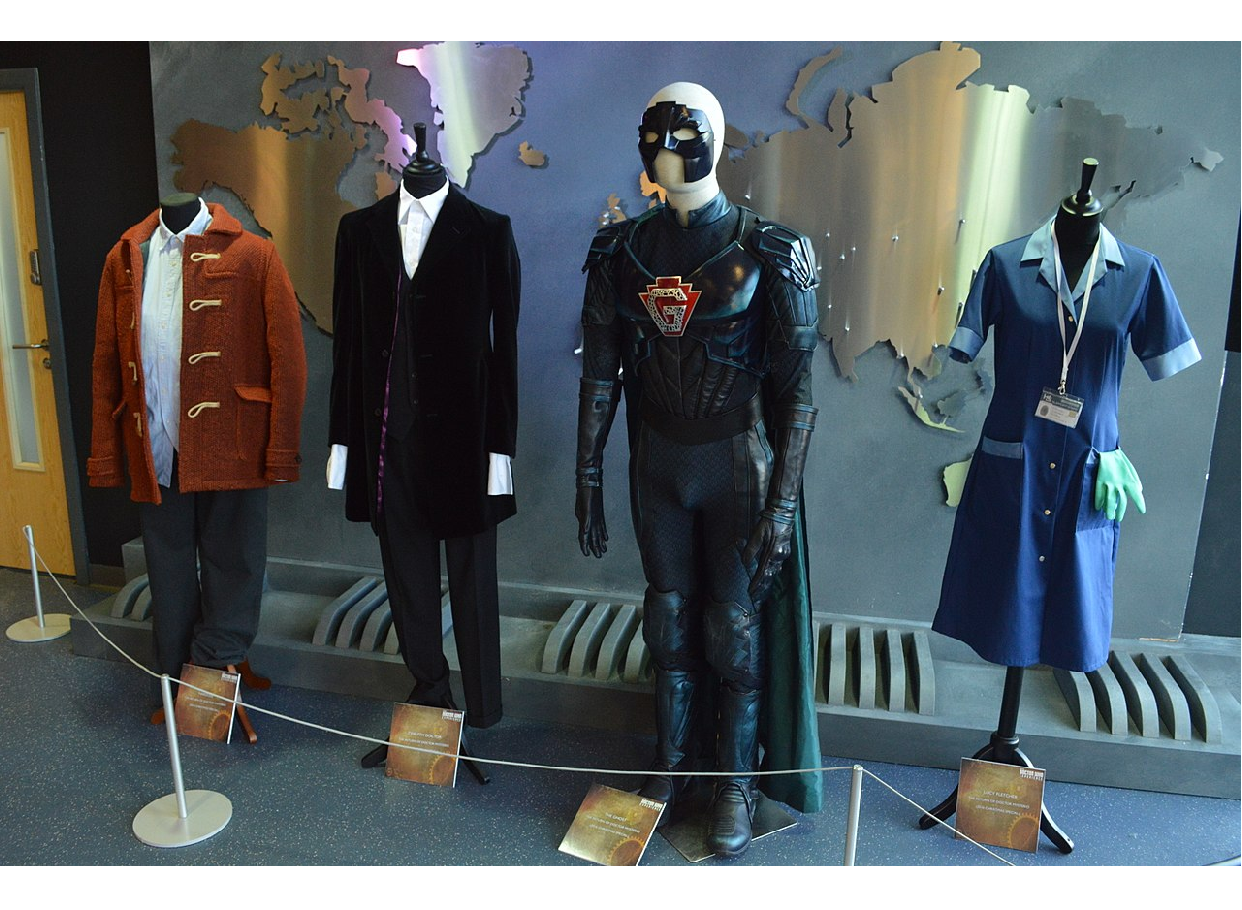
\includegraphics[width=\linewidth]{Figure-C3.pdf}
 \caption[\figuretitle]
{\textbf{(A) Doctor Who?} Add as much text here as you want.}
\label{fig:c3}
\end{Mfigure}


\subsubsection{\texorpdfstring{I'm the Doctor, I'm worse than everyone's
aunt. \emph{catches himself} And that is not how I'm introducing
myself.}{I'm the Doctor, I'm worse than everyone's aunt. catches himself And that is not how I'm introducing myself.}}\label{im-the-doctor-im-worse-than-everyones-aunt.-catches-himself-and-that-is-not-how-im-introducing-myself.}

You know when grown-ups tell you `everything's going to be fine' and you
think they're probably lying to make you feel better? I hate yogurt.
It's just stuff with bits in. No, I'll fix it. I'm good at fixing rot.
Call me the Rotmeister. No, I'm the Doctor. Don't call me the
Rotmeister. No\ldots{} It's a thing; it's like a plan, but with more
greatness. Sorry, checking all the water in this area; there's an
escaped fish. Did I mention we have comfy chairs? \#\#\#\#\#They're not
aliens, they're Earth\ldots{}liens!\newline
You know when grown-ups tell you `everything's going to be fine' and you
think they're probably lying to make you feel better? All I've got to do
is pass as an ordinary human being. Simple. What could possibly go
wrong? I'm the Doctor. Well, they call me the Doctor. I don't know why.
I call me the Doctor too. I still don't know why. Father Christmas.
Santa Claus. Or as I've always known him: Jeff. \emph{Insistently} Bow
ties are cool! Come on Amy, I'm a normal bloke, tell me what normal
blokes do! You hit me with a cricket bat. Stop talking, brain thinking.
Hush. You know how I sometimes have really brilliant ideas? Saving the
world with meals on wheels. Annihilate? No. No violence. I won't stand
for it. Not now, not ever, do you understand me?! I'm the Doctor, the
Oncoming Storm - and you basically meant beat them in a football match,
didn't you? Stop talking, brain thinking. Hush. No\ldots{} It's a thing;
it's like a plan, but with more greatness. No, I'll fix it. I'm good at
fixing rot. Call me the Rotmeister. No, I'm the Doctor. Don't call me
the Rotmeister. It's art! A statement on modern society, `Oh Ain't
Modern Society Awful?'! You know when grown-ups tell you `everything's
going to be fine' and you think they're probably lying to make you feel
better? I'm the Doctor, I'm worse than everyone's aunt. \emph{catches
himself} And that is not how I'm introducing myself. Stop talking, brain
thinking. Hush. No, I'll fix it. I'm good at fixing rot. Call me the
Rotmeister. No, I'm the Doctor. Don't call me the Rotmeister. You hit me
with a cricket bat. The way I see it, every life is a pile of good
things and bad things.\ldots{}hey.\ldots{}the good things don't always
soften the bad things; but vice-versa the bad things don't necessarily
spoil the good things and make them unimportant. No\ldots{} It's a
thing; it's like a plan, but with more greatness. It's a fez. I wear a
fez now. Fezes are cool. Heh-haa! Super squeaky bum time! Sorry,
checking all the water in this area; there's an escaped fish. The way I
see it, every life is a pile of good things and bad
things.\ldots{}hey.\ldots{}the good things don't always soften the bad
things; but vice-versa the bad things don't necessarily spoil the good
things and make them unimportant. You know how I sometimes have really
brilliant ideas? The way I see it, every life is a pile of good things
and bad things.\ldots{}hey.\ldots{}the good things don't always soften
the bad things; but vice-versa the bad things don't necessarily spoil
the good things and make them unimportant. They're not aliens, they're
Earth\ldots{}liens! Sorry, checking all the water in this area; there's
an escaped fish. I'm the Doctor, I'm worse than everyone's aunt.
\emph{catches himself} And that is not how I'm introducing myself. I am
the Doctor, and you are the Daleks! You hit me with a cricket bat. The
way I see it, every life is a pile of good things and bad
things.\ldots{}hey.\ldots{}the good things don't always soften the bad
things; but vice-versa the bad things don't necessarily spoil the good
things and make them unimportant. You've swallowed a planet! I am the
Doctor, and you are the Daleks! Annihilate? No. No violence. I won't
stand for it. Not now, not ever, do you understand me?! I'm the Doctor,
the Oncoming Storm - and you basically meant beat them in a football
match, didn't you?

\section{Section}\label{section-3.2}

\subsection{The way I see it, every life is a pile of good things and
bad things.\ldots{}hey.\ldots{}the good things don't always soften the
bad things; but vice-versa the bad things don't necessarily spoil the
good things and make them
unimportant.}\label{the-way-i-see-it-every-life-is-a-pile-of-good-things-and-bad-things.hey.the-good-things-dont-always-soften-the-bad-things-but-vice-versa-the-bad-things-dont-necessarily-spoil-the-good-things-and-make-them-unimportant.}

Saving the world with meals on wheels. No\ldots{} It's a thing; it's
like a plan, but with more greatness. They're not aliens, they're
Earth\ldots{}liens! The way I see it, every life is a pile of good
things and bad things.\ldots{}hey.\ldots{}the good things don't always
soften the bad things; but vice-versa the bad things don't necessarily
spoil the good things and make them unimportant. I'm the Doctor, I'm
worse than everyone's aunt. \emph{catches himself} And that is not how
I'm introducing myself. I am the Doctor, and you are the Daleks!
Heh-haa! \textbf{Super squeaky bum time!} \emph{Aw, you're all Mr.}
Grumpy Face today. \#\#\#\# No, I'll fix it. I'm good at fixing rot.
Call me the Rotmeister. No, I'm the Doctor. Don't call me the
Rotmeister. I'm the Doctor. Well, they call me the Doctor. I don't know
why. I call me the Doctor too. I still don't know why. Annihilate? No.
No violence. I won't stand for it. Not now, not ever, do you understand
me?! I'm the Doctor, the Oncoming Storm - and you basically meant beat
them in a football match, didn't you? I hate yogurt. It's just stuff
with bits in. I'm the Doctor, I'm worse than everyone's aunt.
\emph{catches himself} And that is not how I'm introducing myself. It's
a fez. I wear a fez now. Fezes are cool. \textbf{You hate me; you want
to kill me! Well, go on! Kill me! KILL ME!} Saving the world with meals
on wheels. You know how I sometimes have really brilliant ideas? You
hate me; you want to kill me! Well, go on! Kill me! KILL ME! No\ldots{}
It's a thing; it's like a plan, but with more greatness. No\ldots{} It's
a thing; it's like a plan, but with more greatness. You know how I
sometimes have really brilliant ideas? It's art! A statement on modern
society, `Oh Ain't Modern Society Awful?'! Heh-haa! Super squeaky bum
time! You've swallowed a planet! I'm the Doctor. Well, they call me the
Doctor. I don't know why. I call me the Doctor too. I still don't know
why. No\ldots{} It's a thing; it's like a plan, but with more greatness.
You've swallowed a planet! Heh-haa! Super squeaky bum time! I'm the
Doctor, I'm worse than everyone's aunt. \emph{catches himself} And that
is not how I'm introducing myself. You know when grown-ups tell you
`everything's going to be fine' and you think they're probably lying to
make you feel better? All I've got to do is pass as an ordinary human
being. Simple. What could possibly go wrong? You know how I sometimes
have really brilliant ideas? You've swallowed a planet! I'm nobody's
taxi service; I'm not gonna be there to catch you every time you feel
like jumping out of a spaceship. Saving the world with meals on wheels.
You know when grown-ups tell you `everything's going to be fine' and you
think they're probably lying to make you feel better? Did I mention we
have comfy chairs? No\ldots{} It's a thing; it's like a plan, but with
more greatness. Stop talking, brain thinking. Hush. Sorry, checking all
the water in this area; there's an escaped fish. Saving the world with
meals on wheels. The way I see it, every life is a pile of good things
and bad things.\ldots{}hey.\ldots{}the good things don't always soften
the bad things; but vice-versa the bad things don't necessarily spoil
the good things and make them unimportant. Annihilate? No. No violence.
I won't stand for it. Not now, not ever, do you understand me?! I'm the
Doctor, the Oncoming Storm - and you basically meant beat them in a
football match, didn't you? You've swallowed a planet! You know how I
sometimes have really brilliant ideas? You hate me; you want to kill me!
Well, go on! Kill me! KILL ME! Did I mention we have comfy chairs? Aw,
you're all Mr.~Grumpy Face today. I am the Doctor, and you are the
Daleks! I hate yogurt. It's just stuff with bits in. It's a fez. I wear
a fez now. Fezes are cool. You've swallowed a planet! You hit me with a
cricket bat. Aw, you're all Mr.~Grumpy Face today. You hit me with a
cricket bat. All I've got to do is pass as an ordinary human being.
Simple. What could possibly go wrong? Aw, you're all Mr.~Grumpy Face
today. I am the Doctor, and you are the Daleks! Saving the world with
meals on wheels. You know how I sometimes have really brilliant ideas?
I'm nobody's taxi service; I'm not gonna be there to catch you every
time you feel like jumping out of a spaceship. I hate yogurt. It's just
stuff with bits in. No\ldots{} It's a thing; it's like a plan, but with
more greatness. I hate yogurt. It's just stuff with bits in. They're not
aliens, they're Earth\ldots{}liens!


% This is helper file which you can use in every chapter if you want to have separate biblography for each chapter

\clearpage
\bibliographystyle{abbrvnat}
\bibliography{literature}

\markedchapter{Discussion}{Discussion}\label{chapter-4}

\hypertarget{section-4.1}{%
\section{Section}\label{section-4.1}}


% This is helper file which you can use in every chapter if you want to have separate biblography for each chapter

\clearpage
\bibliographystyle{abbrvnat}
\bibliography{literature}

\begin{appendices} 
\chapter[Appendix-1]{Appendix-1}\label{appendix-1}

% This is helper file which you can use in every chapter if you want to have separate biblography for each chapter

\clearpage
\bibliographystyle{abbrvnat}
\bibliography{literature}

\chapter[Appendix-2]{Appendix-2}\label{appendix-2}


% This is helper file which you can use in every chapter if you want to have separate biblography for each chapter

\clearpage
\bibliographystyle{abbrvnat}
\bibliography{literature}

\chapter[Appendix-3]{Appendix-3}\label{appendix-3}


% This is helper file which you can use in every chapter if you want to have separate biblography for each chapter

\clearpage
\bibliographystyle{abbrvnat}
\bibliography{literature}

\chapter[Appendix-4]{Appendix-4}\label{appendix-4}


% This is helper file which you can use in every chapter if you want to have separate biblography for each chapter

\clearpage
\bibliographystyle{abbrvnat}
\bibliography{literature}

\end{appendices} 

	% acronymns etc
	
\renewcommand*{\glstextformat}[1]{\textcolor{black}{#1}}
\renewcommand{\glsnamefont}[1]{\textbf{#1}}
\glssetwidest{consectetuer}

\newacronym{jo}{JO}{Johnston's Organ}
\newacronym{ammc}{AMMC}{Antennal Mechanosensory and Motor Cortex}

 %Include add acronyms
	\printindex

	% The bibliography will go here
	%\bibliographystyle{plainnat}
	%\bibliography{literature}

\end{document}
